\section{Theoretisch Kader}
In dit hoofdstuk wordt informatie verzameld en concepten behandel voor het realiseren van het sluis model.

\subsection{De Kripke structuur}

Kripke structuren zijn een manier om het gedrag van een systeem te modelleren. Belangrijke termen voor het bespreken van Kripke structuren zijn states en transities. \newline

Een state beschrijft de toestand waarin een systeem zich bevindt. In het geval dat de state niet duidelijk is voor de gebruiker dan wordt dat mode confusion genoemd. Transities zijn de overgangen van één state naar de anderen. 

\begin{figure}[!h]
	\centering
	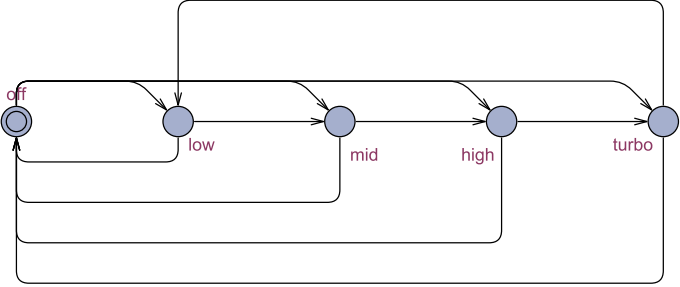
\includegraphics[width=\textwidth]{kripke_structure_example1}
    \caption{Voorbeeld Kripke structuur}
	%\label{fig:figure2}
\end{figure}

\subsection{Soorten modellen} \label{SoortenModellen}

\textbf{World vs. machine:} 
\\
Er kan onderscheid worden gemaakt tussen de fenomenen die zich bevinden in de wereld buiten het systeem en de fenomenen die alleen in het systeem zelf bestaan. Deze verschillen verschilt voor elke machine, het hangt volledig af van welke inputs en outputs de machine heeft. Een simpele voorbeeld van wereldse fenomeen is het temperatuur en een fenomeen die alleen in het machine bestaat is het programma waar het machine op functioneert. \\\\
\textbf{4 variabelen methode:}
\\
Modellen voor computer systemen gebruiken vaak antropomorfisme analogie en intuïtieve conclusies wat tot lager precisie kan leiden. Het vier variabelen model helpt om software vereisten met groter precisie vast te stellen, door deze te modelleren op een manier zoals vaak door ingenieurs wordt toegepast. \cite{parnas1995functional} 
\\\\
Zoals de naam suggereert bestaat het vier variabelen model uit vier onderdelen. Input, output, gecontroleerde variabelen en gemonitorde variabelen. Als eerste de gemonteerde variabelen die buiten het systeem bestaan en worden opgenomen door sensoren, waarna deze input is voor de software. Deze input draagt bij aan de output of acties die het systeem in de buitenwereld creëert, de resultaten hiervan heten de gecontroleerde variabelen. Zie ook Figuur ~\ref{fig:four_Variables} hieronder.


\begin{figure}[!h]
	\centering
	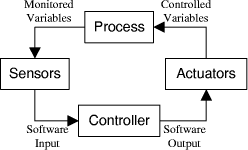
\includegraphics[width=\textwidth]{four_Variables}
    \caption{Vier variabelen model \cite{thompson2000requirements}}
	\label{fig:four_Variables}
\end{figure}

\subsection{Tijd}
In Uppaal wordt tijd globaal op hetzelfde tempo bijgehouden. Tijd wordt in klokken bijgehouden en kan op elk moment worden uitgelezen of gereset. Tijd in uppaal heeft geen vaste eenheid en er kunnen verschillende eenheden toegewezen worden zolang het wek consistent word uitgevoerd. \cite{uppaalsmalltutorial}
\subsection{Guards en invarianten}
Guards zijn condities die op transities worden geplaatst, aan deze condities moet worden voldaan voordat deze transitie mogelijk is. Een van de vele condities die je kan definiëren is het verstrijken van een bepaalde eenheid tijd voordat het die transitie mag aan ingaan. \cite{uppaalsmalltutorial}

\subsection{Deadlock} \label{deadlock}

Een deadlock is een situatie waarin er nooit meer verdere state transities mogelijke zijn. Dit zorgt ervoor dat het systeem volledig stil staat en niks meer kan doen. Deadlocks kunnen ontstaan door door bepaalde condities te definiëren die het systeem niet kan waarmaken \cite{uppaalintro}.

\subsection{Zeno gedrag} \label{zenobehavior}
Wanneer een model een oneindig aantal transities kan maken in een bepaalde tijd dat wordt er gesproken van zeno gedrag. \cite{uppaaltutorialmodelingpatterns} \cite{leine2011zeno}.

\subsection{Waterniveau}

In een document waarin informatie over de vaarwegen in Nederland zijn verzameld, is een standaard aangehouden van 2,45 meter en 1,10 meter voor respectievelijk de doorvaarthoogte en diepte \cite{vaarwegennederland2017}. 